%%%%%%%%%%%%%%%%%%%%%%%%%%%%%%%%%%%%%%%%%
% Beamer Presentation
% LaTeX Template
% Version 1.0 (10/11/12)
%
% This template has been downloaded from:
% http://www.LaTeXTemplates.com
%
% License:
% CC BY-NC-SA 3.0 (http://creativecommons.org/licenses/by-nc-sa/3.0/)
%
%%%%%%%%%%%%%%%%%%%%%%%%%%%%%%%%%%%%%%%%%

 
%----------------------------------------------------------------------------------------
%	PACKAGES AND THEMES
%----------------------------------------------------------------------------------------

\documentclass[15pt]{beamer}
\usepackage[utf8]{inputenc}
\usepackage{amsmath}
\usepackage{graphicx}
\usepackage{hyperref}
\usepackage{float}
\usepackage{wrapfig}
\usepackage[french]{babel}
\usepackage{comment} % enables the use of multi-line comments (\ifx \fi) 
\usepackage{lipsum} %This package just generates Lorem Ipsum filler text.
\usepackage[final]{pdfpages} 
%\usepackage[french]{babel}
\pdfmapfile{+sansmathaccent.map}

\mode<presentation> {

% The Beamer class comes with a number of default slide themes
% which change the colors and layouts of slides. Below this is a list
% of all the themes, uncomment each in turn to see what they look like.

%\usetheme{default}
%\usetheme{AnnArbor}
%\usetheme{Antibes}
%\usetheme{Bergen}
%\usetheme{Berkeley}
%\usetheme{Berlin}
%\usetheme{Boadilla}
%\usetheme{CambridgeUS}
%\usetheme{Copenhagen}
%\usetheme{Darmstadt}
%\usetheme{Dresden}
%\usetheme{Frankfurt}
%\usetheme{Goettingen}
%\usetheme{Hannover}
%\usetheme{Ilmenau}
%\usetheme{JuanLesPins}
%\usetheme{Luebeck}
\usetheme{Madrid}
%\usetheme{Malmoe}
%\usetheme{Marburg}
%\usetheme{Montpellier}
%\usetheme{PaloAlto}
%\usetheme{Pittsburgh}
%\usetheme{Rochester}
%\usetheme{Singapore}
%\usetheme{Szeged}
%\usetheme{Warsaw}

% As well as themes, the Beamer class has a number of color themes
% for any slide theme. Uncomment each of these in turn to see how it
% changes the colors of your current slide theme.

%\usecolortheme{albatross}
\usecolortheme{beaver}
%\usecolortheme{beetle}
%\usecolortheme{crane}
%\usecolortheme{dolphin}
%\usecolortheme{dove}
%\usecolortheme{fly}
%\usecolortheme{lily}
%\usecolortheme{orchid}
%\usecolortheme{rose}
%\usecolortheme{seagull}
%\usecolortheme{seahorse}
%\usecolortheme{whale}
%\usecolortheme{wolverine}

%\setbeamertemplate{footline} % To remove the footer line in all slides uncomment this line
\setbeamertemplate{footline}[page number] % To replace the footer line in all slides with a simple slide count uncomment this line

%\setbeamertemplate{navigation symbols}{} % To remove the navigation symbols from the bottom of all slides uncomment this line
}

\usepackage{graphicx} % Allows including images
\usepackage{booktabs} % Allows the use of \toprule, \midrule and \bottomrule in tables


\def \stg {stream graph}
\def \Stgs {Stream graphs}
\def \Stg {Stream graph}
\def \stgm {stream graph multicouches}
\def \Stgm {Stream graph multicouches}
\def \stgs {stream graphs}
\def \stgms {stream graphs multicouches}
\def \Stgms {Stream graphs multicouches}

%tikz 
\usepackage{tikz}
\usepackage{pgfplots}
\usepackage{amsmath}
\usetikzlibrary{decorations.pathmorphing, positioning}
\definecolor{echoreg}{HTML}{2cb1e1}
\definecolor{echodrk}{HTML}{0099cc}
\tikzstyle{mybox} = [text=black, very thick,
    rectangle, rounded corners, inner sep=10pt, inner ysep=20pt]
\tikzstyle{fancytitle} =[text=black]
\newcommand{\yslant}{0.5}
\newcommand{\xslant}{-0.6}

%%%%%%%%%%%%%%%%%%%%%%%%%%%%%%%% TIKZ STYLES
\tikzstyle{every node}=[font=\scriptsize]

\tikzset{RootStyle/.style = {
						shape          = circle,
			      draw           = red!50!black!50,
			      thick,
			      top color      = white,
			      bottom color   = red!50!black!20,
			      text           = black,
			      inner sep      = .2pt,
			      outer sep      = 0pt,
			      minimum size   = 2.5 mm}
						}

\tikzset{VertexStyle/.style = {
						shape          = circle,
			      draw           = black!50,
			      top color      = white,
			      bottom color   = black!20,
			      text           = black,
			      inner sep      = .2pt,
			      outer sep      = 0pt,
			      minimum size   = 1.75 mm}
						}

\tikzset{EdgeStyle/.style   = {thick,<->}}

\tikzset{LabelStyle/.style =   {
				  text           = black,
				  inner sep      = .2pt,
				  outer sep      = 1pt,
				  font           =\scriptsize,
				  minimum size   = 2.15 mm}
					}

\pgfplotsset{compat=1.15}

\newcommand\overmat[3]{%
  \makebox[0pt][l]{$\smash{\color{#3}\overbrace{\phantom{%
    \begin{matrix}#2\end{matrix}}}^{\text{#1}}}$}#2}
\newcommand\undermat[3]{%
  \makebox[0pt][l]{$\smash{\color{#3}\underbrace{\phantom{%
    \begin{matrix}#2\end{matrix}}}_{\text{#1}}}$}#2}
\newcommand\partialphantom{\vphantom{\frac{\partial e_{P,M}}{\partial w_{1,1}}}}


%----------------------------------------------------------------------------------------
%	TITLE PAGE
%----------------------------------------------------------------------------------------

\title{\Stgms{}} % The short title appears at the bottom of every slide, the full title is only on the title page
\subtitle{Soutenance de stage de recherche}
\author{Pimprenelle Parmentier (X16) \\ Stage de recherche\\ Riken AIP} % Your name

%\logo{} 
\date{} 
\subject{}



\begin{document}

\begin{frame}
\titlepage % Print the title page as the first slide

\textbf{Tuteurs :} \\
Tiphaine Viard {\footnotesize(Riken AIP)}\\
Benjamin Renoust {\scriptsize(Institute for Datability Science}, {\footnotesize Osaka University)}\\
Jean-François Baffier {\footnotesize(JSPS)}


\end{frame}

\begin{frame}{Plan}
    \tableofcontents
\end{frame}

%\begin{frame}
%\frametitle{Plan} % Table of contents slide, comment this block out to remove it
%\tableofcontents % Throughout your presentation, if you choose to use \section{} and \subsection{} commands, these will automatically be printed on this slide as an overview of your presentation
%\end{frame}

\section*{Introduction}
\begin{frame}{Introduction}
\textbf{Graphes} : relations (liens, arêtes) entre des individus (noeuds, sommets).
\[
	G=(V,E)
\]
\pause
\begin{minipage}{0.4\linewidth}
{\large Quelques exemples :}
\begin{itemize}
    \item relations sociales
    \item réseau IP
    \item réseaux de transports
\end{itemize}
\end{minipage}
\pause
\begin{minipage}{0.5\linewidth}
\begin{figure}
	\centering
    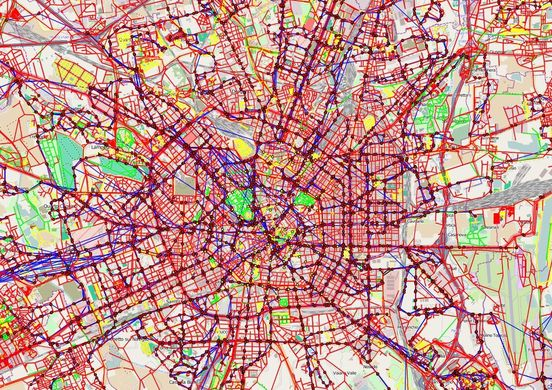
\includegraphics[width=\textwidth]{img/multimodalTransport.jpg}
\end{figure}
\end{minipage}
\pause

$\Rightarrow$ {\large Comment prendre en compte...}
\begin{itemize}
	\item des n\oe{}uds et des arêtes de natures différentes ?
    \item des interactions qui dépendent du temps ?
\end{itemize}
\end{frame}

\section{Présentation de l'objet mathématique}
\subsection{Méthodologie}
\begin{frame}{Méthodologie}
	\begin{itemize}
		\item utile : \begin{itemize}
							\item applicable
							\item resultats exploitables
						\end{itemize}		 \pause
		\item efficace \begin{itemize}
							\item manipulable \og facilement \fg{} : unifier les notations
							\item complexité optimale
						\end{itemize}\pause
		\item cohérent \pause
		\item généralisation de l'existant : 
			\begin{itemize}
				\item graphes multicouches
				\item \stgs{}
			\end{itemize}
	\end{itemize}
\end{frame}

\subsection{Graphes multicouches}
\begin{frame}{Graphes multicouches : structures complexes}

\begin{minipage}{0.4\textwidth}
	$$\mathbf{M=(V_M,E_M,V,L)}$$
\begin{footnotesize}
$V = \{A,B,C,D\}$\\
$L = \{$milieu, type de relation$\}$\\
$V_M = \{(A,[$forêt,combat$]), \dots \}$\\
$E_M = \{$Arêtes entre les éléments de $V_M \}$
\end{footnotesize}
\end{minipage}
\begin{minipage}[r]{0.59\textwidth}
\begin{figure}
    \flushright
    
%0.58
\begin{tikzpicture}[scale=0.38,every node/.style={minimum size=1cm},on grid]

	\node [mybox, scale=1.0] at (10.5, 2) (box){%
		\begin{minipage}{0.6\textwidth}
			
    	\end{minipage}
	};
	
	
	% etage 2
	\begin{scope}[
		yshift=-210,
		every node/.append style={yslant=\yslant,xslant=\xslant},
		yslant=\yslant,xslant=\xslant
	] 
		%\draw[black, dashed, thin] (0,0) rectangle (7,7); 
		\fill[olive,fill opacity=.75] (0,0) rectangle (7,7);
		
		\fill[orange,fill opacity=.75] (10,0) rectangle (17,7);
		%\draw[black, dashed, thin] (10,0) rectangle (17,7); 
		
		\draw[fill=echoreg]  %foret, collabo
			(5,2) node(111){} circle (.1) %A
			(2,2) circle (.1) %B
			(2,5) circle (.1); %C
			%(5,5) circle (.1); %D
		
		\draw[fill=echoreg]  %plaine, collabo
			(15,2) node(111){} circle (.1) %A
			%(12,2) circle (.1) %B
			(12,5) circle (.1) %C
			(15,5) circle (.1); %D
		 
		\draw[ thin, color=echodrk]%foret collab
			(2,4.9) to (2,2.1); %C->B
		\draw[ thin, color=echodrk]
			(2.1,2) to (4.9,2);%B->A
		
		\draw[thin, color=echodrk]%plaine collab
			(12,5) to (15,2);%C->A
		\draw[thin, color=echodrk]
			(12,5) to (15,5);
			
		\fill[black]
			(0.5,6.5) node[right, scale=.7] {Forêt, Collaboration}	
			(5.1,1.9) node[right,scale=.7]{\bf A}
			(1.9,1.9) node[left,scale=.7]{\bf B}
			(2,5.2) node[left,scale=.7]{\bf C};
			%(5.2,5.1) node[right,scale=.7]{\bf D}; 
			
		\fill[black]
			(10.5,6.5) node[right, scale=.7] {Plaine, Collaboration}	
			(15.1,1.9) node[right,scale=.7]{\bf A}
			%(11.9,1.9) node[left,scale=.7]{\bf B}
			(12,5.2) node[left,scale=.7]{\bf C}
			(15.2,5.1) node[right,scale=.7]{\bf D}; 
		
		
	\end{scope}
	
	% Interlayer crossconnections
	% vertical
	\draw[thick,  dashed, decorate] (3.8, 4) to (3.8, -3.5);%A
	\draw[thick, dashed, decorate] (.8,2.4) to (.8,-5);%B
	\draw[thick,  dashed, decorate] (-1, 4.5) to (-1, -2.8);%C
	
1	\draw[thick,  dashed, decorate] (13.8,9) to (13.8, 1.5);%A
	\draw[thick, dashed, decorate] (12,11) to (12,3.6);%D
	\draw[thick,  dashed, decorate] (9, 9.5) to (9, 2.1);%c
	
	%horizontal
	
	
	\draw[thick, dashed, decorate] (-1,-2.8) to[bend left] (9,2.1);
	\draw[thick, dashed, decorate] (3.8,-3.5) to[bend left] (13.8,1.5);
	
	
	% etage 1
	\begin{scope}[
		yshift=0,
		every node/.append style={yslant=\yslant,xslant=\xslant},
		yslant=\yslant,xslant=\xslant
	]
		\fill[olive,fill opacity=.85] (0,0) rectangle (7,7); 
		%\draw[black, dashed, thin] (0,0) rectangle (7,7); 
		
		\fill[orange,fill opacity=.85] (10,0) rectangle (17,7);
		%\draw[black, dashed, thin] (10,0) rectangle (17,7); 
		
		\draw [fill=red]
			(5,2) node(111){} circle (.1)%A %foret, combat
			(2,2) circle (.1)%B
			(2,5) circle (.1)%C
			(5,5) circle (.1);%D

		\draw[fill=red]  
			(15,2) node(111){} circle (.1) %A % plaine combat
			%(12,2) circle (.1) %B
			(12,5) circle (.1) %C
			(15,5) circle (.1); %D
		
		\draw[thin, color=red]%foret combat
			(2,2.1) to (2,4.9);%B->C
			
		\draw[thin, color=red]%plaine combat
			(12,5) to (15,5);%C->D
		
		
		\fill[black]
			(0.5,6.5) node[right, scale=.7] {Forêt, Combat}
			(5.1,1.9) node[right,scale=.7]{\bf A}
			(1.9,1.9) node[left,scale=.7]{\bf B}
			(1.9,5) node[left,scale=.7]{\bf C}
			(5.2,5.1) node[right,scale=.7]{\bf D}; 
			
		\fill[black]
			(10.5,6.5) node[right, scale=.7] {Plaine, Combat}
			(15.1,1.9) node[right,scale=.7]{\bf A}
			%(11.9,1.9) node[left,scale=.7]{\bf B}
			(12,5.2) node[left,scale=.7]{\bf C}
			(15.2,5.1) node[right,scale=.7]{\bf D};
			
	\end{scope} 
	
	%interlayer
	\draw[thick, dashed, decorate] (-1,4.5) to[bend left] (9,9.5);
	\draw[thick, dashed, decorate] (3.8,4) to[bend left] (13.8,9);
	\draw[thick, dashed, decorate] (2.1,6.1) to[bend left] (12,11);
\end{tikzpicture}

\end{figure}
\end{minipage}
$$
\left.
\begin{array}{l}
    \text{ Différents types d'interactions}\\
    \text{ Différents types de n\oe{}uds}
\end{array}
\right \}\rightarrow \textbf{Structures complexes}
$$

\end{frame}

\subsection{Stream graphs}

\begin{frame}{\Stgs{} : modéliser les interactions dépendant du temps}


\medskip

\begin{minipage}{0.43\textwidth}
\[
	\mathbf{S=(T,V,W,E)}
\]
\begin{footnotesize}
$T=[0,10]$\\
$V=\{A,B,C\}$\\
$W = \{(t,u) | u \text{ existe à t } t\}$\\
$E = \{(t,(u,v)) | (u,v) \text{ existe à t } t\}$
\end{footnotesize}
\end{minipage}
\begin{minipage}[r]{0.55\textwidth}
\begin{figure}
    \flushright
    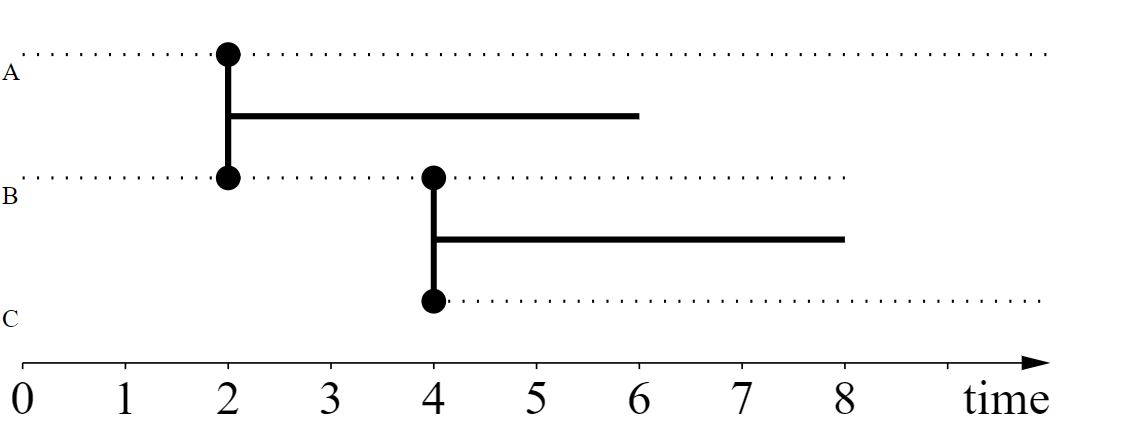
\includegraphics[width=0.8\textwidth]{img/exStreamGraph.JPG}
    \label{fig:exstream}
\end{figure}
\end{minipage}
\medskip

\begin{itemize}
    \item les n\oe{}uds peuvent apparaître et disparaître en fonction du temps
    \item les liens peuvent apparaître et disparaître en fonction du temps
\end{itemize}
\smallskip
\centering
$\rightarrow \textbf{Modélisation d'interactions au cours du temps}$





\end{frame}


\subsection{\Stgms{}}
\begin{frame}{Le \stgm{}}
\[
G=(T,T_M,V,W_M,E_M,\cal{L})
\]

\begin{figure}
    \centering
    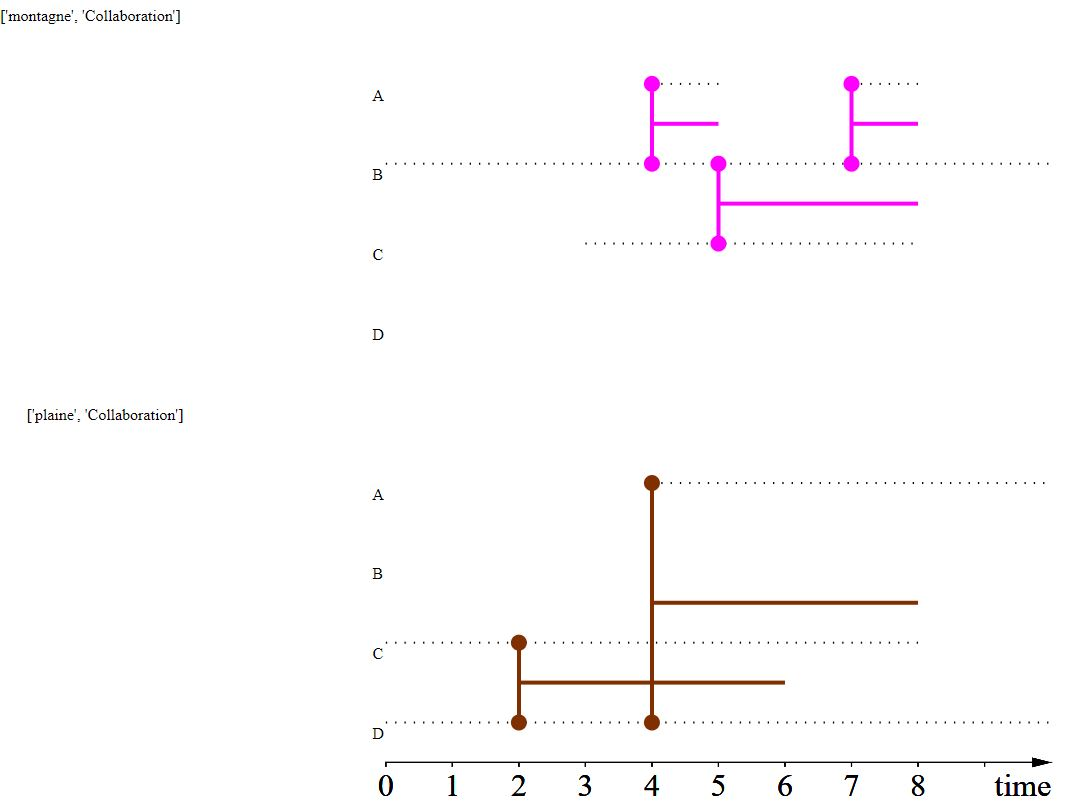
\includegraphics[width=0.7\linewidth]{img/exMultiStream.JPG}
\end{figure}
\end{frame}
\begin{frame}{Le \stgm{}}
	\[
		G=(T,T_M,V,W_M,E_M,\cal{L})
	\]
	\begin{minipage}{0.59\linewidth}
		\begin{figure}
    		\centering
    		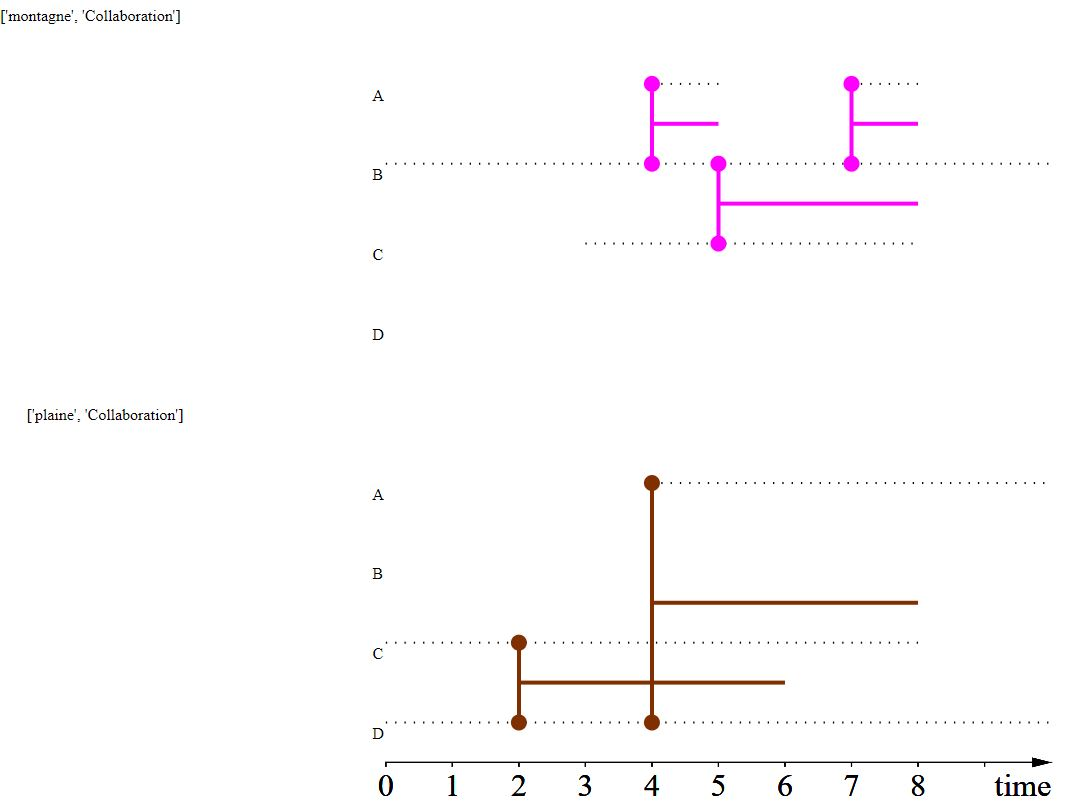
\includegraphics[width=\linewidth]{img/exMultiStream.JPG}
		\end{figure}
	\end{minipage}
	\begin{minipage}{0.4\textwidth}
		\begin{footnotesize}
			$T=[0,10]$\\ \pause
			${\cal L} = \{$milieu,type de relation$\}$\\ \pause
			$V=\{A,B,C,D\}$\\ \pause
			$T_M= \{([0,10],($forêt,Collaboration$)), \dots \}$\pause
		\end{footnotesize}
	\end{minipage}

	\begin{footnotesize}
		$W_M = \{ (t,(A,[$forêt,Collaboration$]))| t \in [4,5]\cup[7,8]), \dots \}$ \pause
		\\
		$E_M= \{ (t,(A,[$plaine,Collaboration),(C,[plaine,Collaboration$])| t \in [4,8]), \dots \}$
	\end{footnotesize}
\end{frame}

\section{Implémentation: bibliothèque et exemples d'utilisation}
\subsection{Une bibliothèque Python pour les \stgms{}}
\begin{frame}{Une bibliothèque Python pour les \stgms{}}
    \begin{figure}
        \centering
        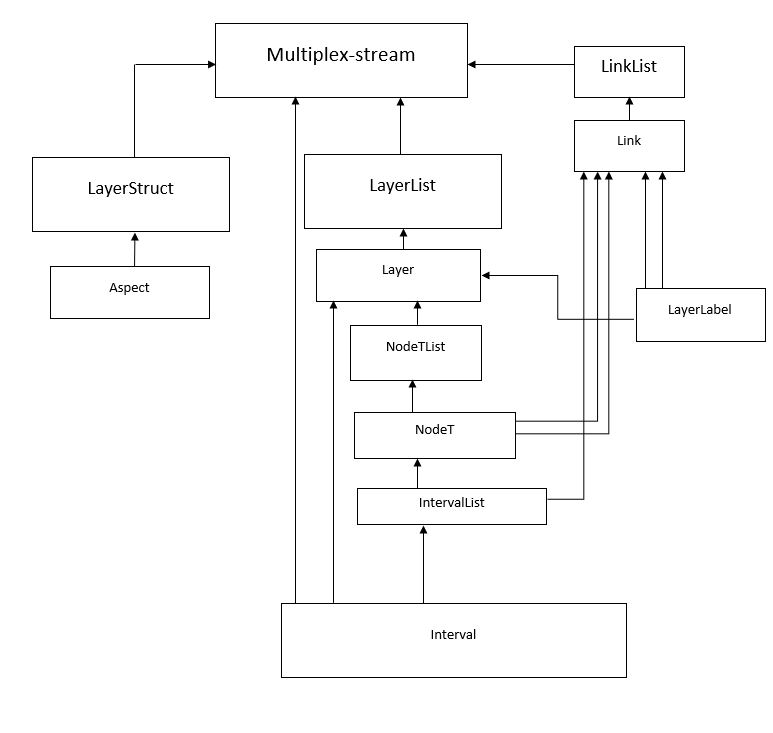
\includegraphics[width=0.7\textwidth]{img/codeStructure.JPG}
        \label{fig:my_label}
    \end{figure}
\end{frame}
\begin{frame}{Jeu de données: interactions entre élèves d'un même lycée}
    \begin{itemize}
        \item durée : 5 jours
        \item fréquence : 20 secondes
        \item nombre de d'élèves (noeuds) : 329
        \item aspects: \begin{itemize}
            \item classes (9)
            \item sexe (M/F)
            \item types de relations : face à face, facebook, amitié
        \end{itemize}
        \item nombre de couches : $2\times 9 \times 3 = 54$
        \item nombre de noeuds-couches : 987
    \end{itemize}
\end{frame}

\subsection{Visualisation}
\begin{frame}{Visualisation}
    \begin{figure}
        \centering
        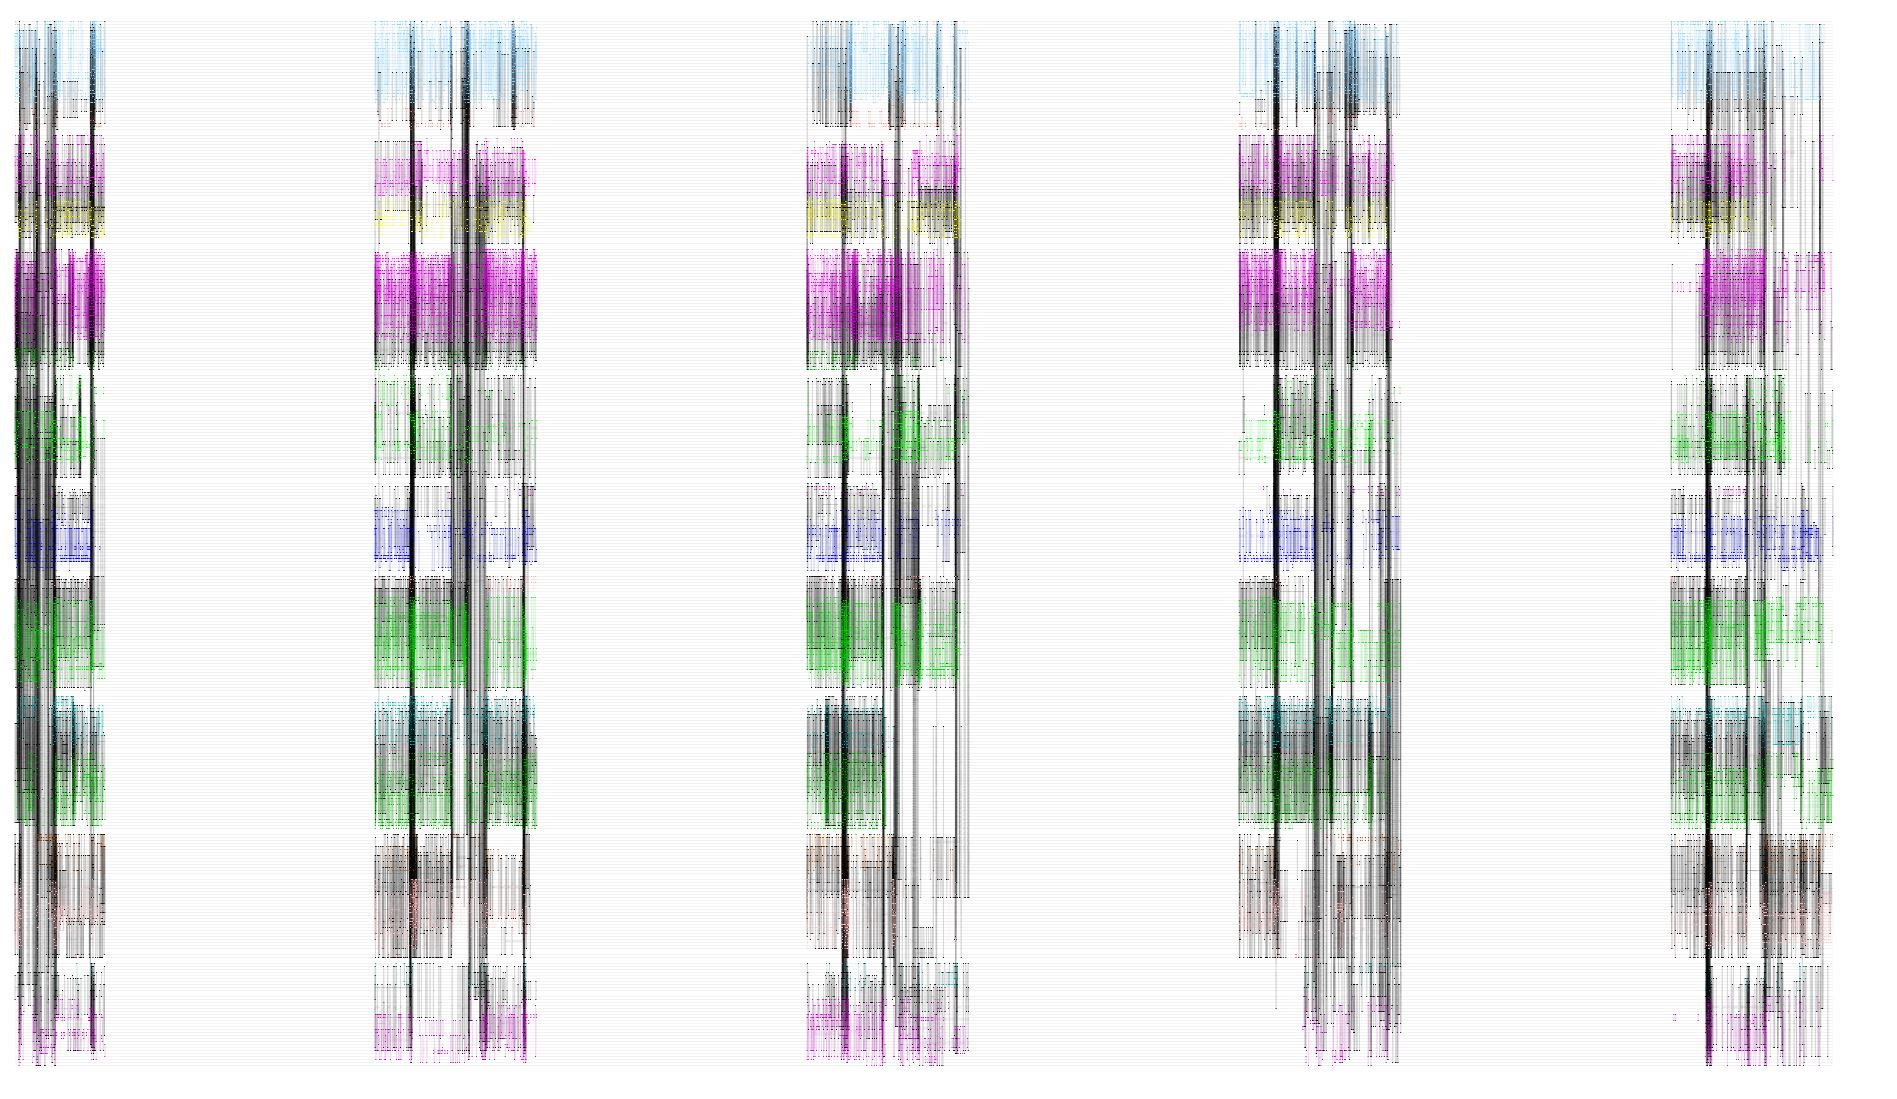
\includegraphics[width=0.9\textwidth]{img/lyceeentier.JPG}
        \caption{Représentation de toutes les interactions sur les 5 jours: en couleurs, les liens intra-couches, en noir, les liens inter-couches.}
        \label{lyceeentier}
    \end{figure}
\end{frame}

\begin{frame}{Visualisation}
    \begin{figure}
        \centering
        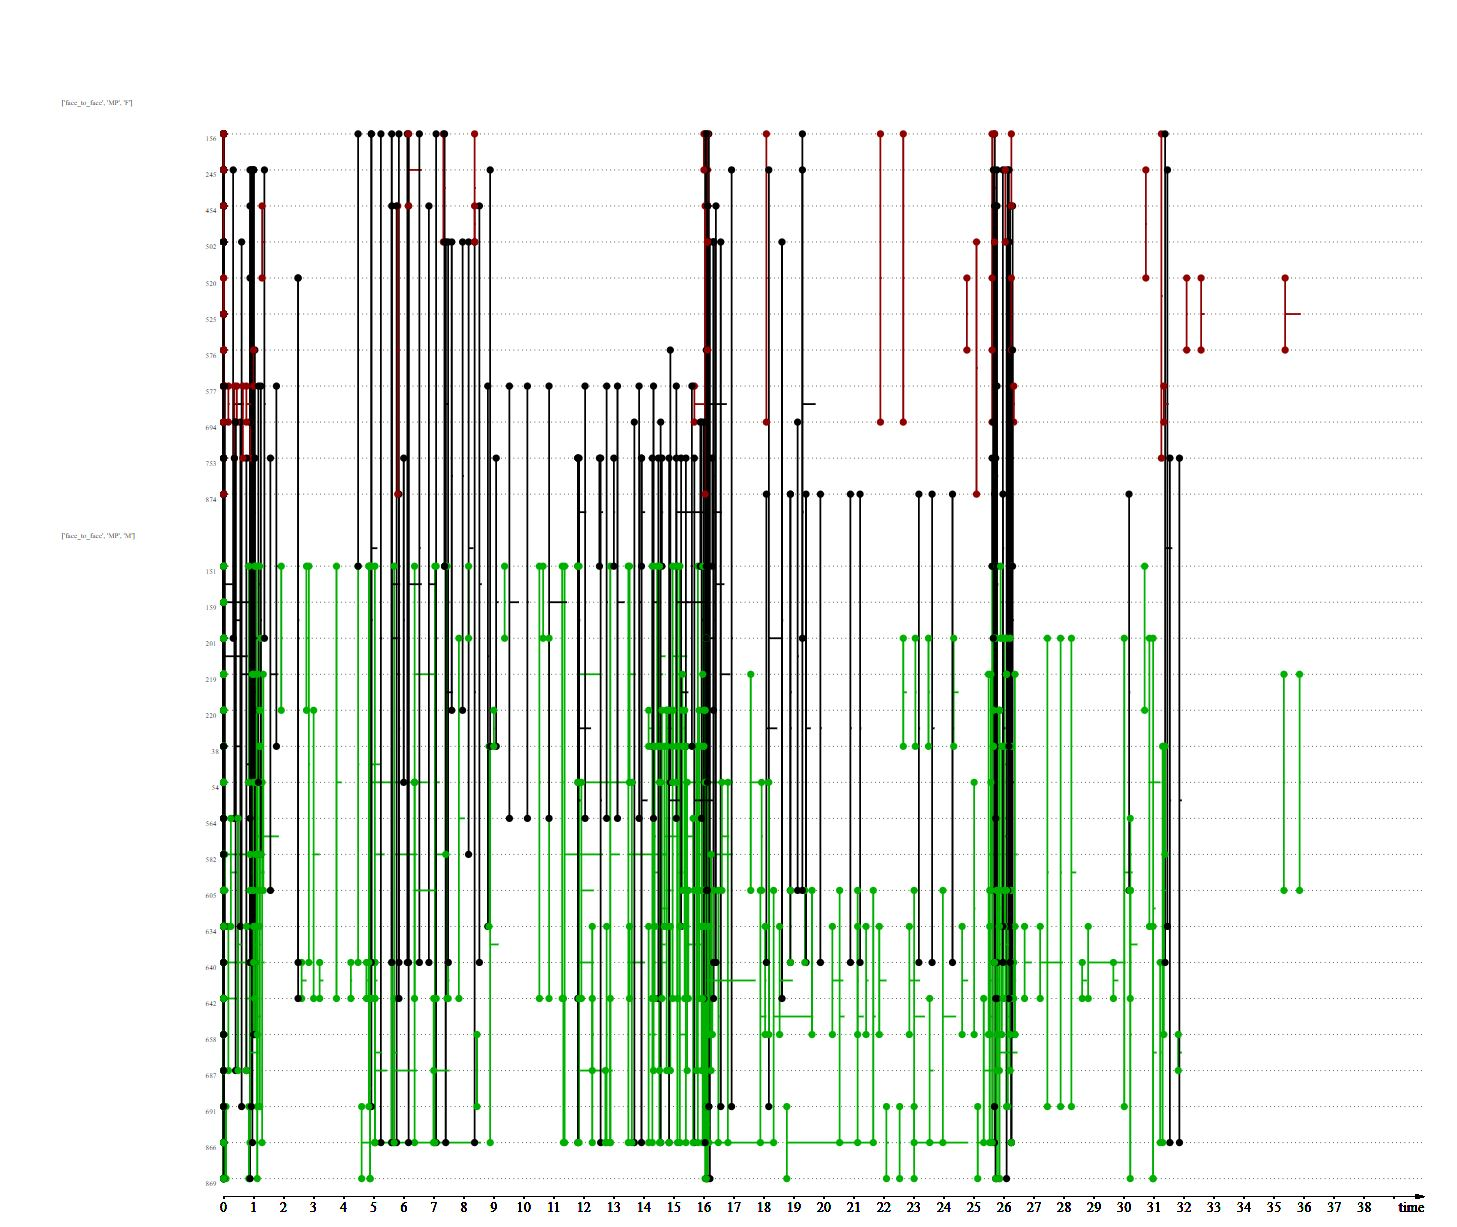
\includegraphics[width=0.6\textwidth]{img/1jourMP.JPG}
        \caption{\og Zoom \fg{} sur la classe de MP le premier jour. En vert les liens intra-couche pour les hommes, en rouge pour les femmes, en noir les liens inter-couches.}
        \label{fig:my_label}
    \end{figure}
\end{frame}

\subsection{Extractions}
\begin{frame}{Extractions : Graphe induit des relations face à face}

\begin{figure}
    \centering
    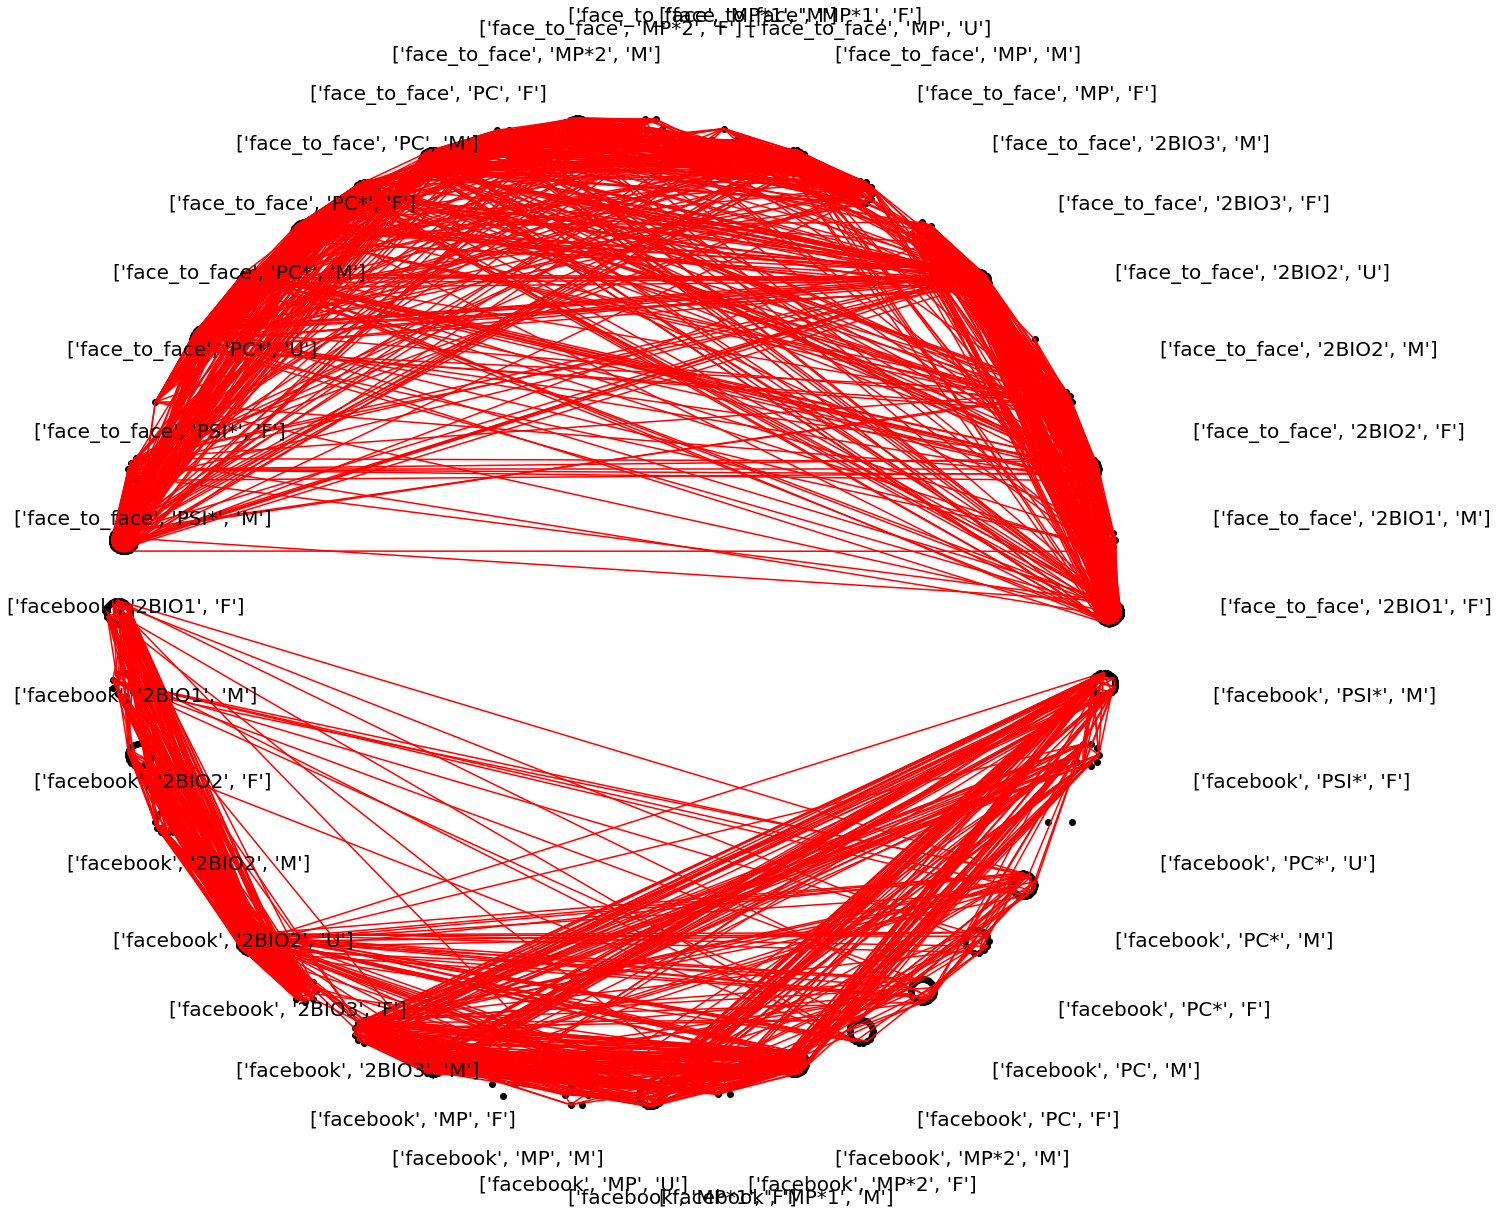
\includegraphics[width=0.5\textwidth]{img/tout.png}
    \caption{Le graphe induit des relations de face à face et facebook.}
    \label{fig:my_label}
\end{figure}
    Le {\em graphe multicouches induit sur l'intervalle $I$} $M_I(S_M) = (V_{M,I}, E_{M,I}, V,L)$ de $S_M$ est le graphe multicouche qui rassemble toutes les couches, n\oe{}uds couches et n\oe{}uds qui apparaissent durant $I$.
    \begin{align*}
    	V_{M,I} = \bigcup_{t\in I} V_{M,t}\\
    	E_{M,I} = \bigcup_{t\in I} E_{M,t}\\
    \end{align*}
\end{frame}

\subsection{Densités}

\begin{frame}{Calcul des densités}
    Densité: probabilité, prenant deux sommets ``joignables", qu'elles soient joins par une arête.
    La {\em densité du \stgm{}} s'écrit: 
	\[
		\delta_M (M) 
		= \frac{\int_{t\in T}|E_M,t|}{\int_{t\in T}|C_t|} 
		= \frac{\sum_{(u,\alpha)(v,\beta) \in E_M}|T_{(u,\alpha)(v,\beta)}|}{|C|}
	\]	
	avec $C=\{$Ensemble des relations possibles$\}$
    
    Ici, $$C=\{(t,(eleve1,[classe1,relation1,sexe1]),$$ $$(eleve2,[classe2,relation2,sexe2])) \text{ avec } relation2=relation1\}$$
\end{frame}

\begin{frame}{Densité d'intérêt dans notre jeu de données}
    Question: la séparation hommes/femmes est-elle \og visible \fg{} dans les relations ?
    
    Calcul des densités:
    \begin{itemize}
        \item densité intra-hommes
        \item densité intra-femmes
        \item densité totale
    \end{itemize}
    $$\delta = \frac{\sum_{u,v \in V\otimes V} |T_{uv}|}{\sum_{u,v \in V \otimes V}|T_u\cap T_v|} = \frac{2|E|}{|T|(|V|(|V|-1))}$$
    \begin{itemize}
        \item densité inter hommes/femmes: graphe biparti
    \end{itemize}
    $$\delta_{biparti}=\frac{\sum_{u,v \in V_f \times V_h} |T_{uv}|}{\sum_{u,v \in V_f \times V_h}|T_u\cap T_v|}=\frac{|E|}{|T||V_f||V_h|}$$
    
\end{frame}

\begin{frame}{Comparaison des densités}
    \begin{figure}
        \centering
        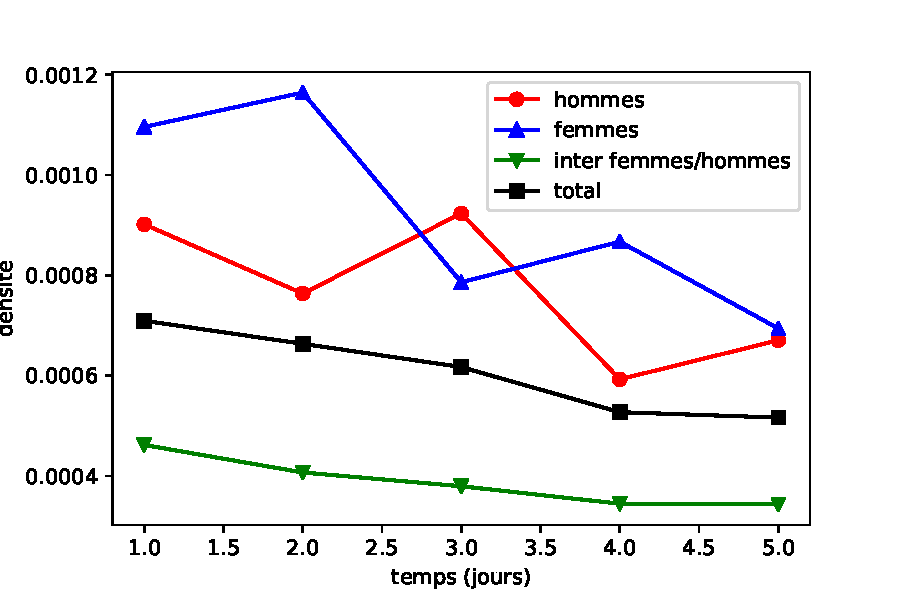
\includegraphics[width=0.8\textwidth]{img/compfg.pdf}
        \caption{Comparatif entre les différentes densités selon le sexe des élèves pour les relations de face à face. On constate qu'en moyenne il y a plus d'interactions intra-sexe qu'inter-sexes.}
        \label{fig:my_label}
    \end{figure}
\end{frame}
    
\begin{frame}{Comparaison des densités en fonction des types de relations}
    
    \begin{figure}
        \centering
        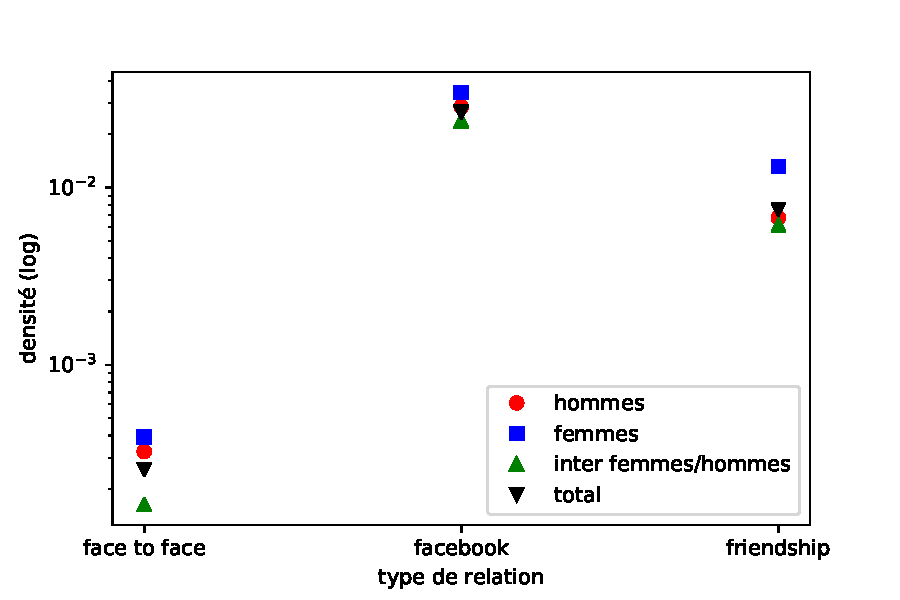
\includegraphics[width=0.8\textwidth]{img/comparatif.pdf}
        \caption{Comparaison des densités entre les différents types d'interactions (echelle logarithmique): la tendance est confirmée dans les autres types de relations }
        \label{fig:my_label}
    \end{figure}
\end{frame}

\begin{frame}{Intérêt de la mesure de densité dans les \stgms{}}
    \begin{minipage}{0.45\textwidth}
        \begin{figure}
            \centering
            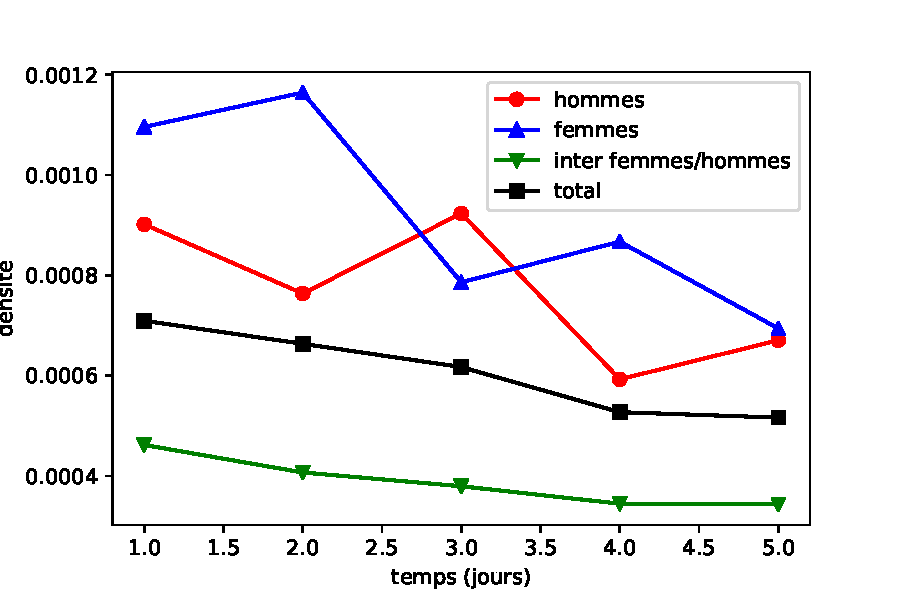
\includegraphics[width=\textwidth]{img/compfg.pdf}
            \caption{Densités dans le \stgm{} des relations de face à face}
            \label{fig:my_label}
        \end{figure}
    \end{minipage}
    \begin{minipage}{0.45\textwidth}
        \begin{figure}
            \centering
            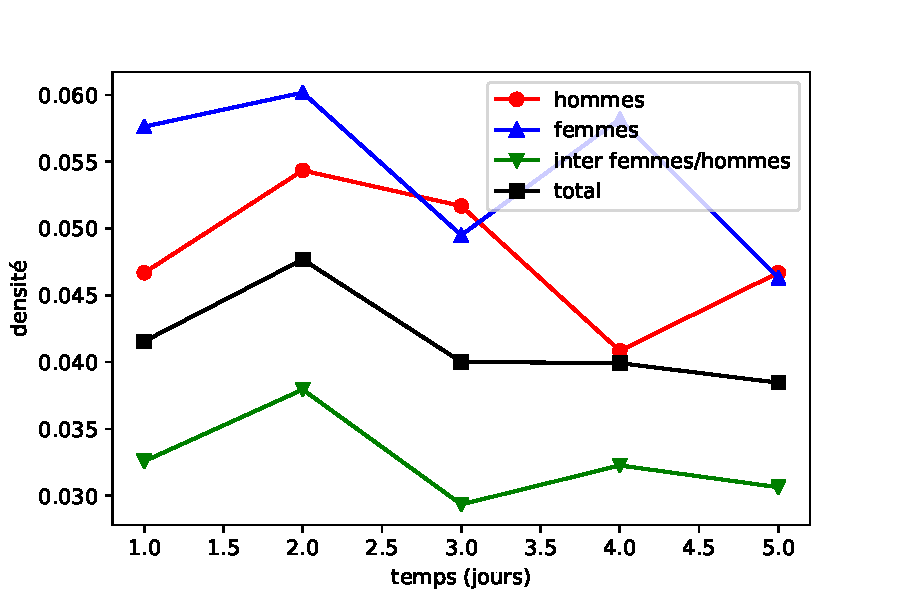
\includegraphics[width=\textwidth]{img/densitesj.pdf}
            \caption{Densités dans le graphe induit des relations de face à face}
            \label{fig:my_label}
        \end{figure}
    \end{minipage}
\end{frame}


\section{Travaux en cours et projets futurs}
\subsection{Ordre des n\oe{}uds}
\begin{frame}{Ordre des n\oe{}uds}
    \textbf{Objectif:} Minimiser les distances entre les n\oe{}uds les plus \og liés \fg{}
    
    
    \textbf{Algorithme:} \begin{itemize}
        \item trier les liens par ordre décroissants de durées
        \item ajouter les n\oe{}uds à une liste en suivant l'ordre des liens
    \end{itemize}
    
    \textbf{A faire:} prouver l'algorithme.
\end{frame}

\begin{frame}{Ordre des n\oe{}uds}
    Avant:
    
    \begin{figure}
        \centering
        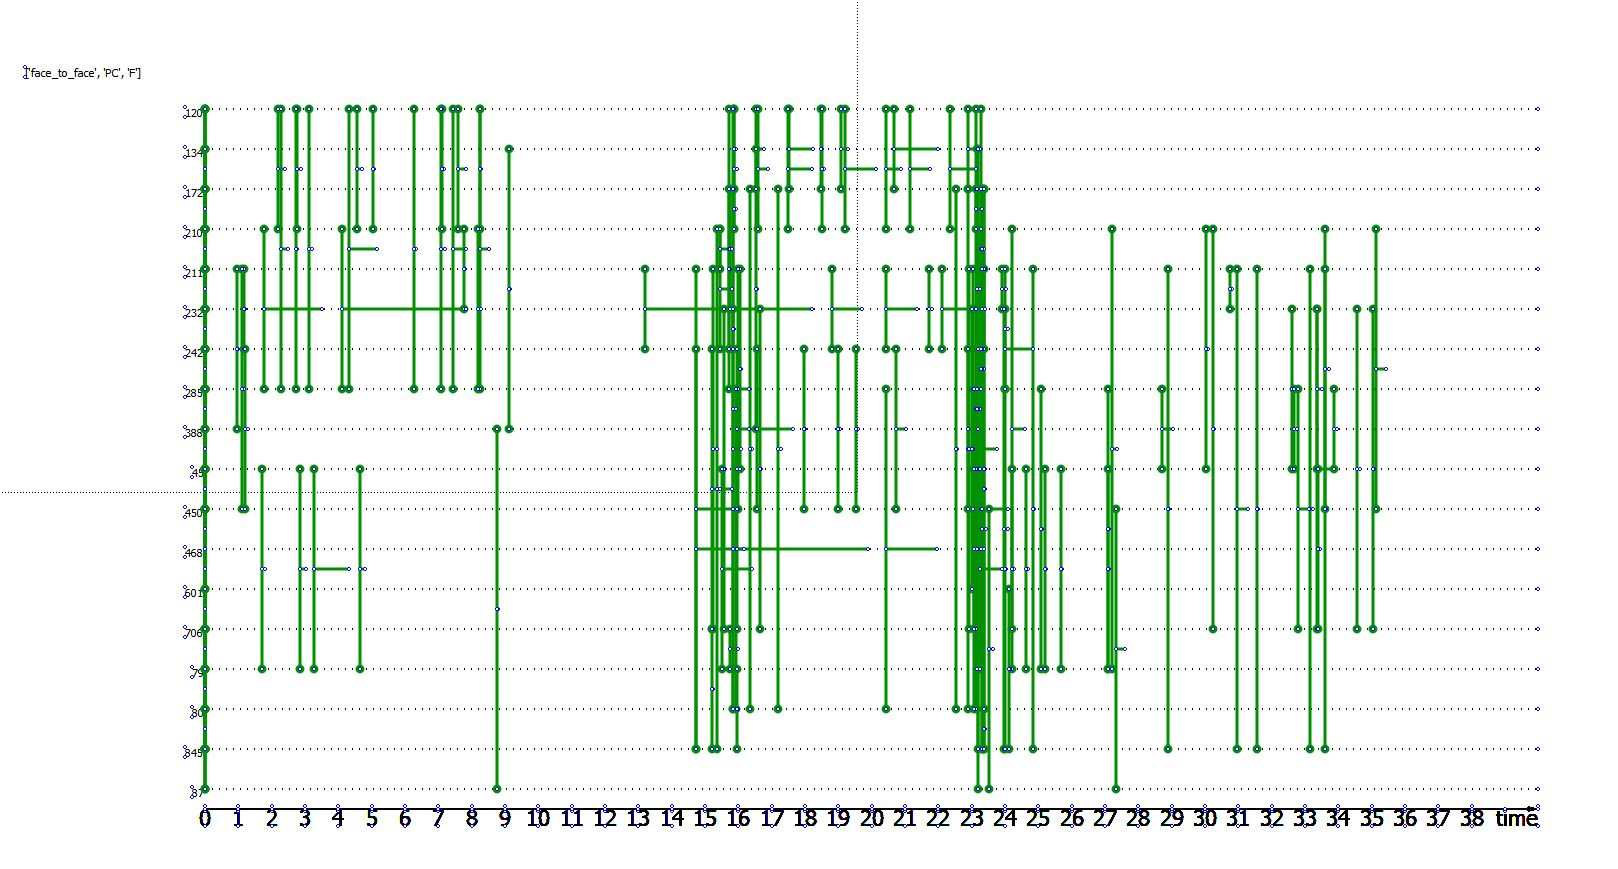
\includegraphics[width=\textwidth]{img/nonordonne.JPG}
        \label{fig:my_label}
    \end{figure}
\end{frame}

\begin{frame}{Ordre des n\oe{}uds}
    Après: 
    
    \begin{figure}
        \centering
        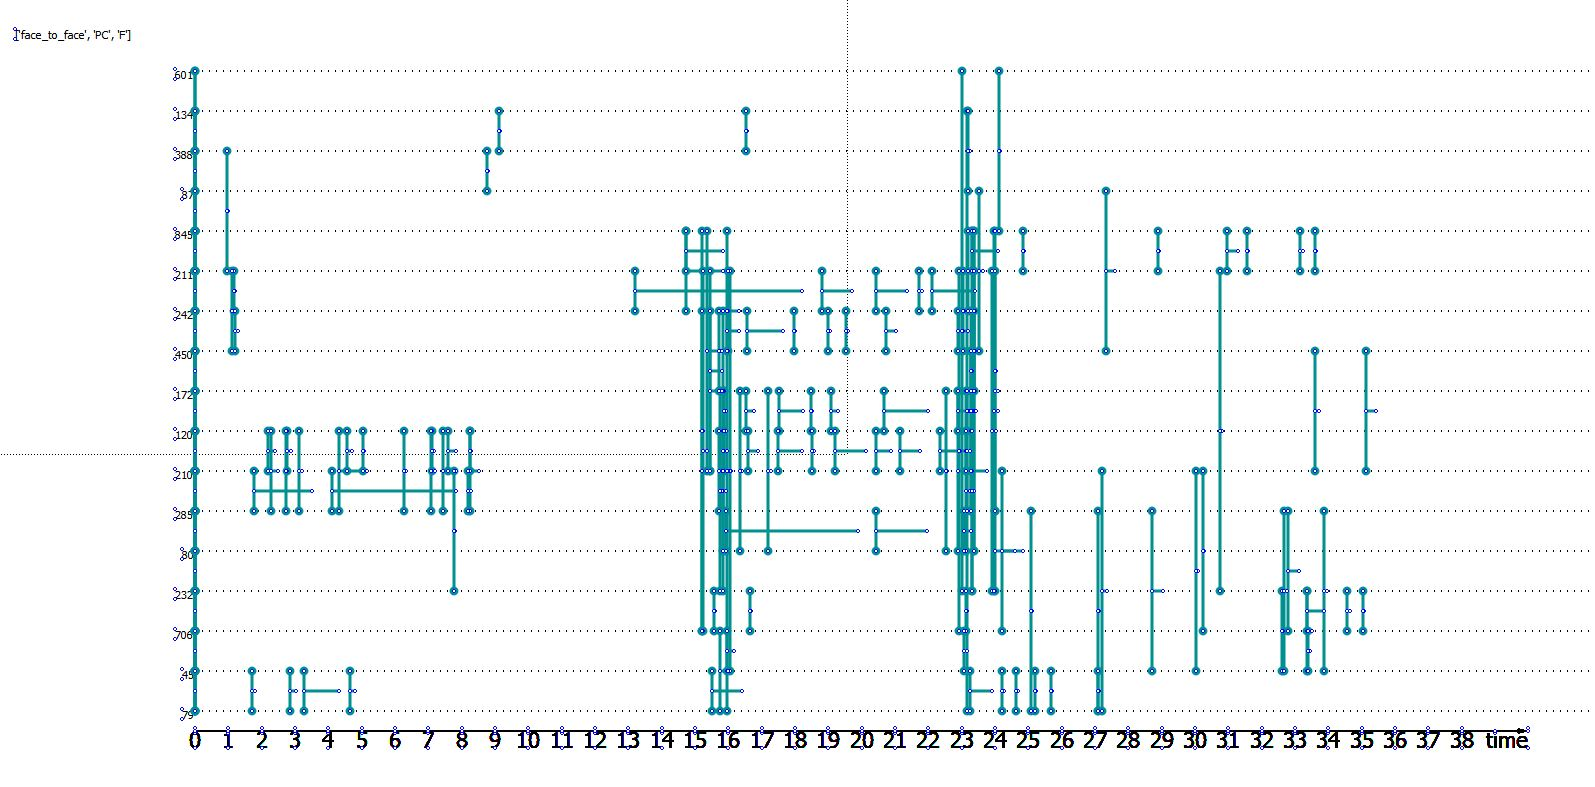
\includegraphics[width=\textwidth]{img/ordonne.JPG}
        \label{fig:my_label}
    \end{figure}
\end{frame}

\subsection{Star Wars et l'intrication }
\begin{frame}{Star Wars et l'intrication}
    \textbf{Star Wars: }
    \begin{itemize}
        \item personnages
        \item mots-clés
        \item lieux 
        \item lien quand deux éléments apparaissent en même temps.
    \end{itemize}
    Problématiques: 
    \begin{itemize}
        \item trouver la répartition en couches la plus adéquate.
        \item calculer une intrication \og temporelle \fg{}
    \end{itemize}
\end{frame}

\subsection{Avions aux US et calculs de diffusion}
\begin{frame}{Avions aux US et calculs de diffusion}
    \textbf{Vols aux États-Unis:}
    \begin{itemize}
        \item n\oe{}uds: aéroports
        \item liens: vols
        \item couches: compagnies aériennes
    \end{itemize}
    Problématiques:
    \begin{itemize}
        \item calculs d'itinéraires
        \item calculs de n\oe{}uds influents
    \end{itemize}
\end{frame}

\begin{frame}{Merci !}
	Résumé: 
	\begin{itemize}
	    \item les \stgms{}, un outil pour modéliser des graphes aux structures complexes, avec une composante temporelle
	    \item extraction de graphes multicouches, de stream graphs et de graphes à partir des \stgms{}
	    \item mesure de la densité
	    \item Pour la suite : ordonnement, intrication et diffusion
	\end{itemize}
\end{frame}

\end{document}
